%
%  progress-presentation.tex
%  src
%
%  Created by Illya Starikov on 09/16/17.
%  Copyright 2017. Illya Starikov. All rights reserved.
%

% \documentclass[notes,xcolor=dvipsnames]{beamer}       % print frame + notes
% \documentclass[notes=only,xcolor=dvipsnames]{beamer}  % only notes
\documentclass[xclolor=dvipsnames]{beamer}            % only frames
%\documentclass[handout,xclolor=dvipsnames]{beamer}    % only frames, no pauses
\usepackage{soul,graphics}

\usepackage{amssymb,amsmath,verbatim,graphicx,microtype,upquote,units,booktabs,akkwidepage}

\newcommand{\chapterNumber}[1]{
    \setcounter{section}{#1}
    \addtocounter{section}{-1}
}
\title{Documentation (Presentation \#5)}
\subtitle{Special Topics (CS3001)}
\author{Illya Starikov}
\date{Sometimes In The Future}
\institute{Missouri University of Science and Technology}

\begin{document}
\begin{darkframes}
    \maketitle

    \begin{frame}
        \frametitle{A Brief Introduction}

        One of the most critical aspects of computer science is documentation.
    \end{frame}

    \begin{frame}
        \frametitle{A Brief Introduction}

        \begin{figure}[H]
            \centering
            
\includegraphics[height=0.8\textheight]{assets/documentation-joke.jpg}
            \label{fig:doc-joke}
        \end{figure}
    \end{frame}

    \begin{frame}
        \frametitle{A Brief Introduction}

        \begin{itemize}
            \item Documentation was one of those things discussed once briefly in Introduction to Programming. You were expected to do it, but never really taught how to do it.
            \item One of my classes this semester (Object Oriented Numerical Modeling) require \textit{a lot} of documentation.
            \item Throughout the semester, I wanted to write good, thorough documentation.
        \end{itemize}
    \end{frame}

    \begin{frame}
        \frametitle{Prior Knowledge}

        \begin{itemize}
            \item Mediocre documentation is easy to write.
                \begin{itemize}
                    \item This is the kind of documentation I wrote my freshmen year.
                \end{itemize}

            \item Great documentation is much harder to write.
                \begin{itemize}
                    \item This is documentation I strive to write now.
                \end{itemize}
        \end{itemize}
    \end{frame}


    \begin{frame}
        \frametitle{Tools}
        \begin{itemize}
            \item Often, it's hard to read documentation when it'd directly inside code.
            \item This is why I've picked up Doxygen, a tool to scrap all documentation outside of a codebase.
        \end{itemize}
    \end{frame}

    \begin{frame}
        \frametitle{Tools (Example)}

        \begin{figure}[H]
            \centering
            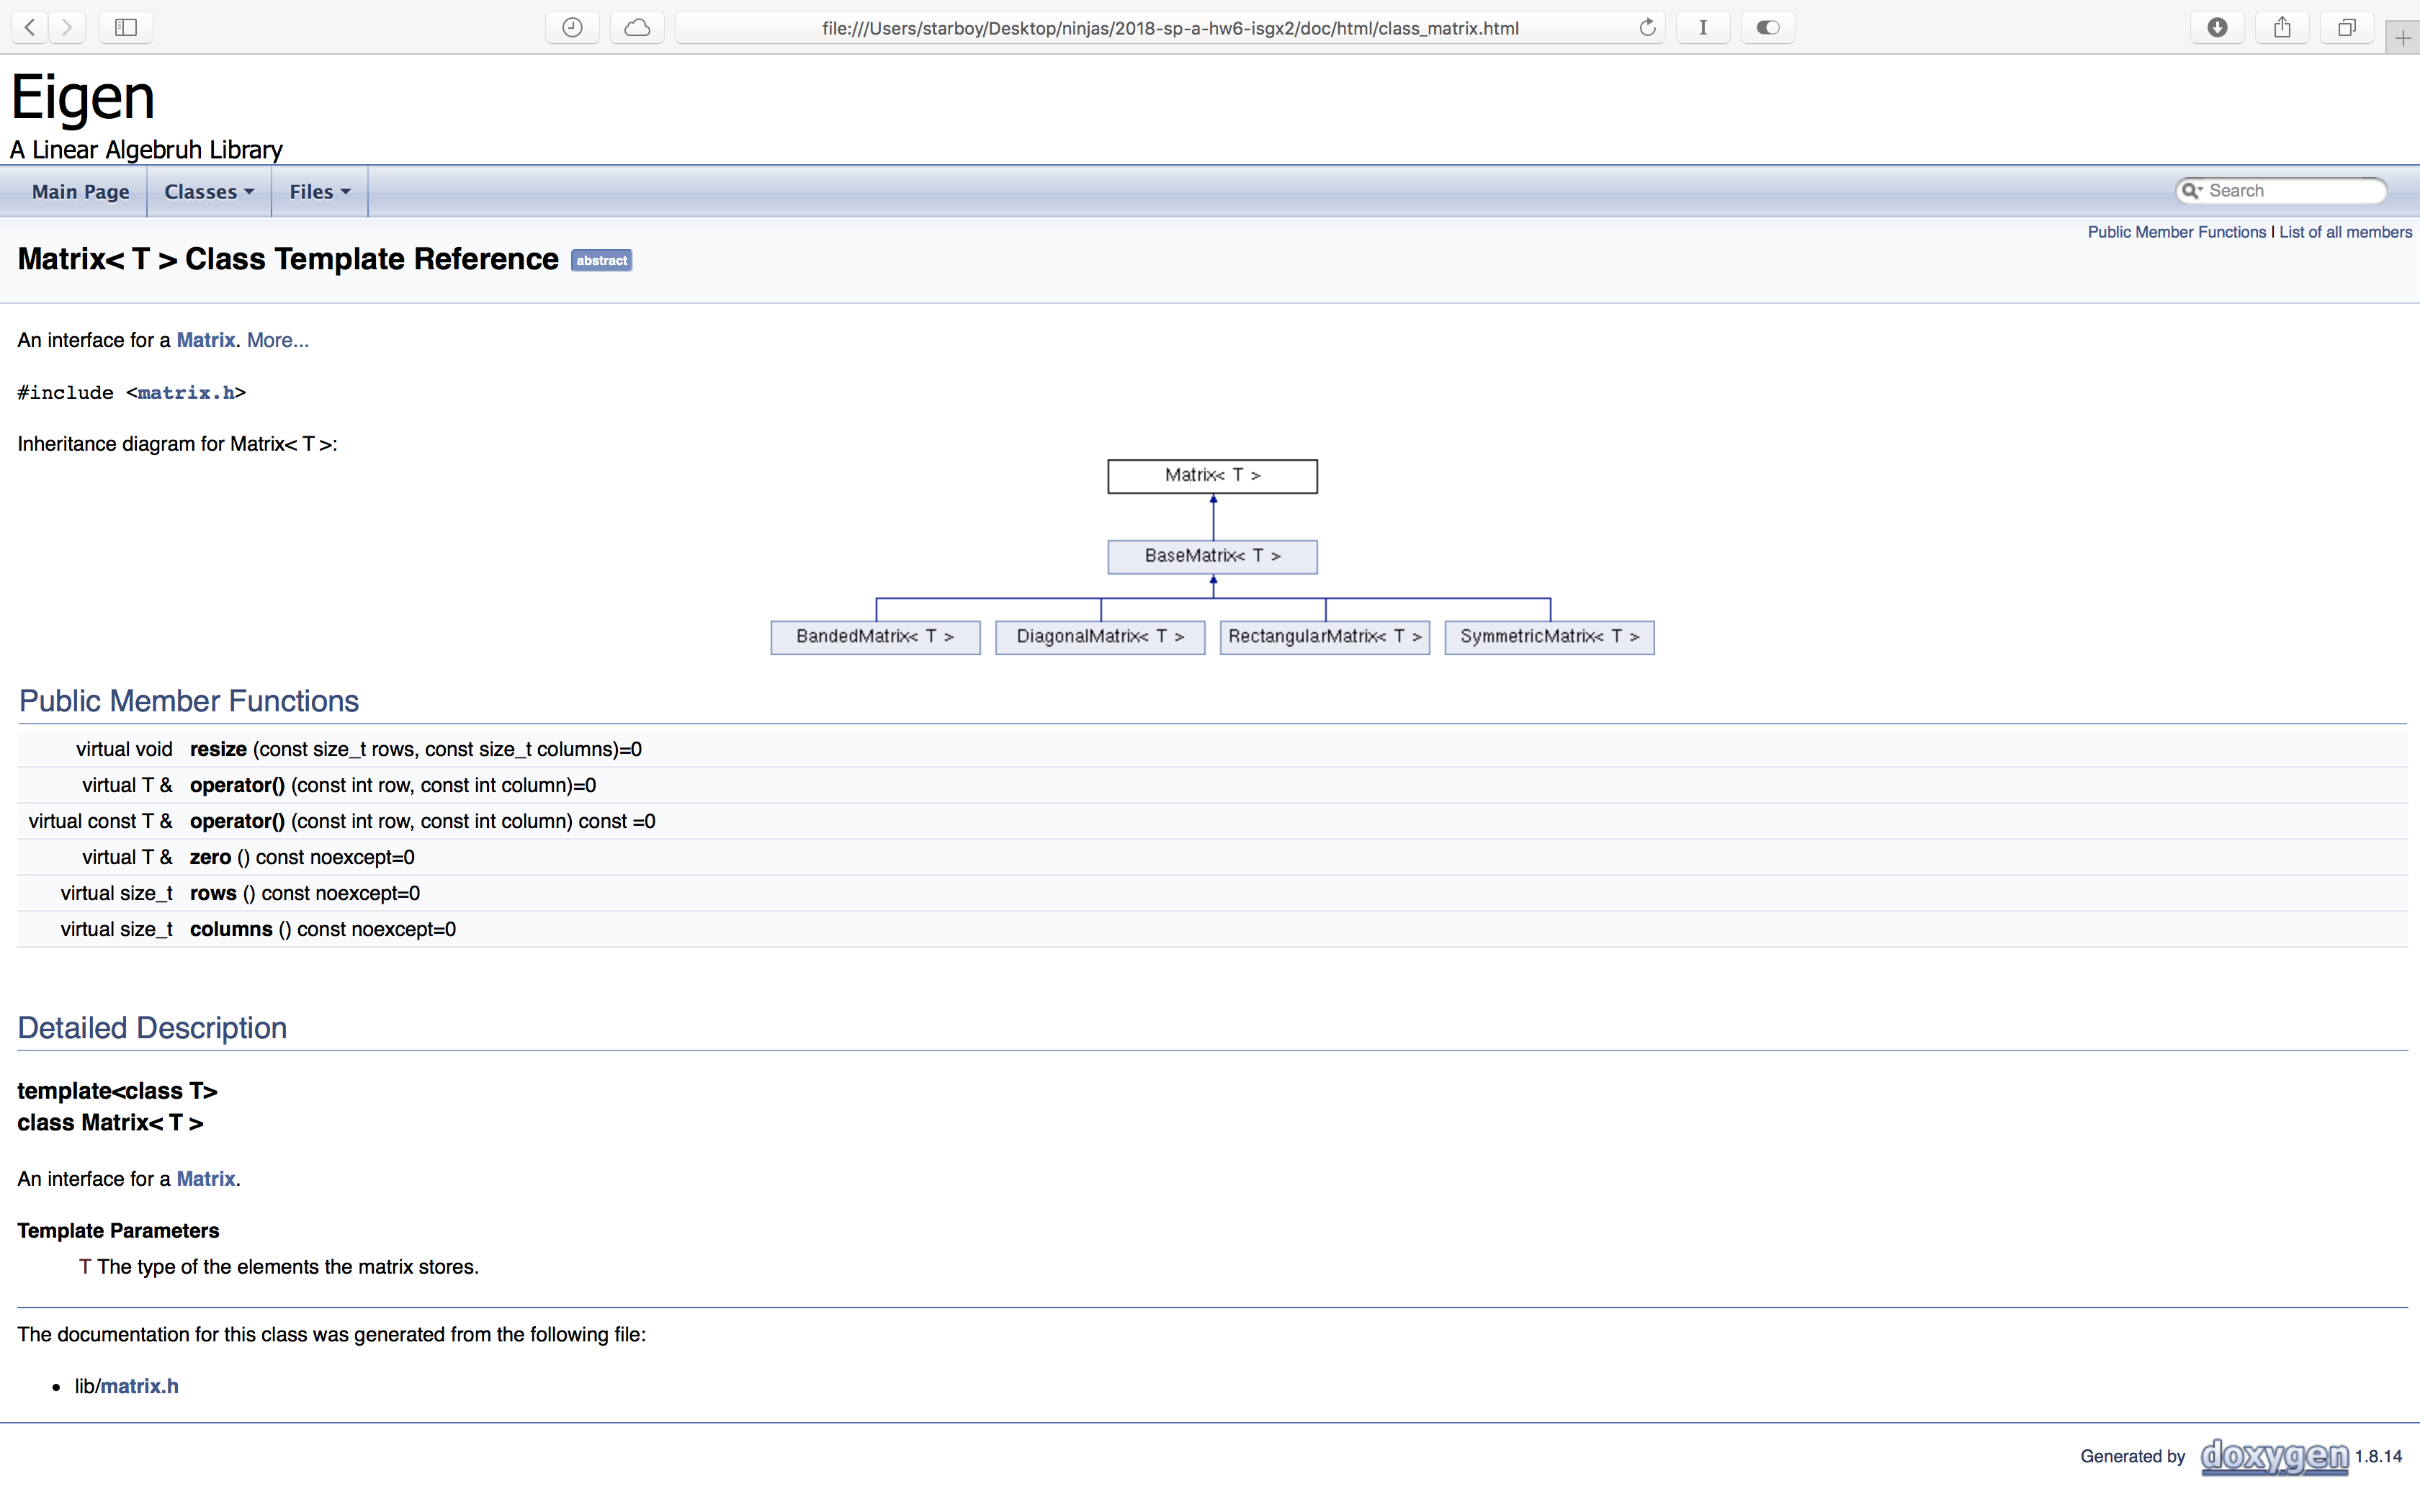
\includegraphics[width=0.95\textwidth]{assets/doxygen.png}
            \label{fig:doxygen}
        \end{figure}

    \end{frame}

    \begin{frame}
        \frametitle{Goals}

        \begin{itemize}
            \item To be able to use Doxygen efficiently.
            \item To write documentation that's easy to read, but also informative.
        \end{itemize}
    \end{frame}

    \begin{frame}[fragile]
        \frametitle{Before --- Intro To Programming}
        \begin{lstlisting}
// Description:     To get user input to dictate what menu option is selected.
// Pre-Condition:   A valid character must be entered.
// Post-Condition:  A value for charMenuOption is received,
// dictating what functions are used form there.
        \end{lstlisting}
    \end{frame}

    \begin{frame}[fragile]
        \frametitle{After --- Object Oriented Numerical Modeling}
        \tiny
        \begin{lstlisting}
/**
 *  @brief Read the specified input file and ensure proper
 *         data format.
 *
 *  @param filename The filename where file is to be read from.
 *         Can be relative or absolute.
 *
 *  @return An `std::string` with the entirety of the file
 *          contents in them (`n` and all).
 *
 *  @warning This does terminate prematurely if the file
 *          contents is not in the proper format.
 **/
        \end{lstlisting}
    \end{frame}

    \begin{frame}
        \frametitle{Resources}

        \begin{itemize}
            \item A great starting point was a \href{http://www-numi.fnal.gov/offline_software/srt_public_context/WebDocs/doxygen-howto.html}{Fermilab introduction article}.

            \item From there, I would reference:
                \begin{itemize}
                    \item \href{https://www.stack.nl/~dimitri/doxygen/results.html}{The doxygen website}.
                    \item \href{https://www.stack.nl/~dimitri/doxygen/manual/commands.html}{The special doxygen command guide}.
                \end{itemize}

            \item I would also read articles about better documentation.
                \begin{itemize}
                    \item \href{https://hackernoon.com/write-good-documentation-6caffb9082b4}{HackerNoon}.
                    \item \href{https://github.com/jamiebuilds/documentation-handbook}{Documentation Handbook}.
                    \item \href{https://news.ycombinator.com/item?id=8414714}{Hacker News}.
                \end{itemize}

        \end{itemize}
    \end{frame}

    \begin{frame}
        \frametitle{Goal Accomplishment}

        \begin{itemize}
            \item So far, this semester, I have only missed two points on documentation for all of my classes.
            \begin{itemize}
                \item Some of my graders even commented on my documentation ability (see attached).
            \end{itemize}
            \item I have been more conscious about my technical writing.
            \item Overall, I saw an improvement in my documentation skills. This is reflected in my school work and my work life.
        \end{itemize}
    \end{frame}

    \begin{frame}
        \frametitle{In Closing}

        All question, comments, and insults can be directed towards me:

        \begin{center}
            \begin{description}
                \item[\faComment] \href{mailto:starikov@mst.edu}{starikov@mst.com}
                \item[\faLinkedin] \href{https://www.linkedin.com/in/illyastarikov/}{Illya Starikov}
                \item[\faGithub] \href{https://github.com/IllyaStarikov/}{Illya Starikov}
                \item[\faRss] \href{https://freneticarray.com/}{FreneticArray.com}
            \end{description}
        \end{center}
    \end{frame}
\end{darkframes}
\end{document}
